\chapter{Visualisierung der Koeffezienten sowie des Taylorpolynoms}
Das resultierende Polynom \(p\left(x\right)\) welches mittels der Gauß'elemination gefunden wurde
ist in Abbildung \ref{fig:TaylorVsGauss} dargestellt. Wie zu sehen ist, oszilliert diese Lösung sehr
stark und ist somit unbrauchbar.

\begin{figure}[H]
    \vspace{-1em}
    \begin{center}
        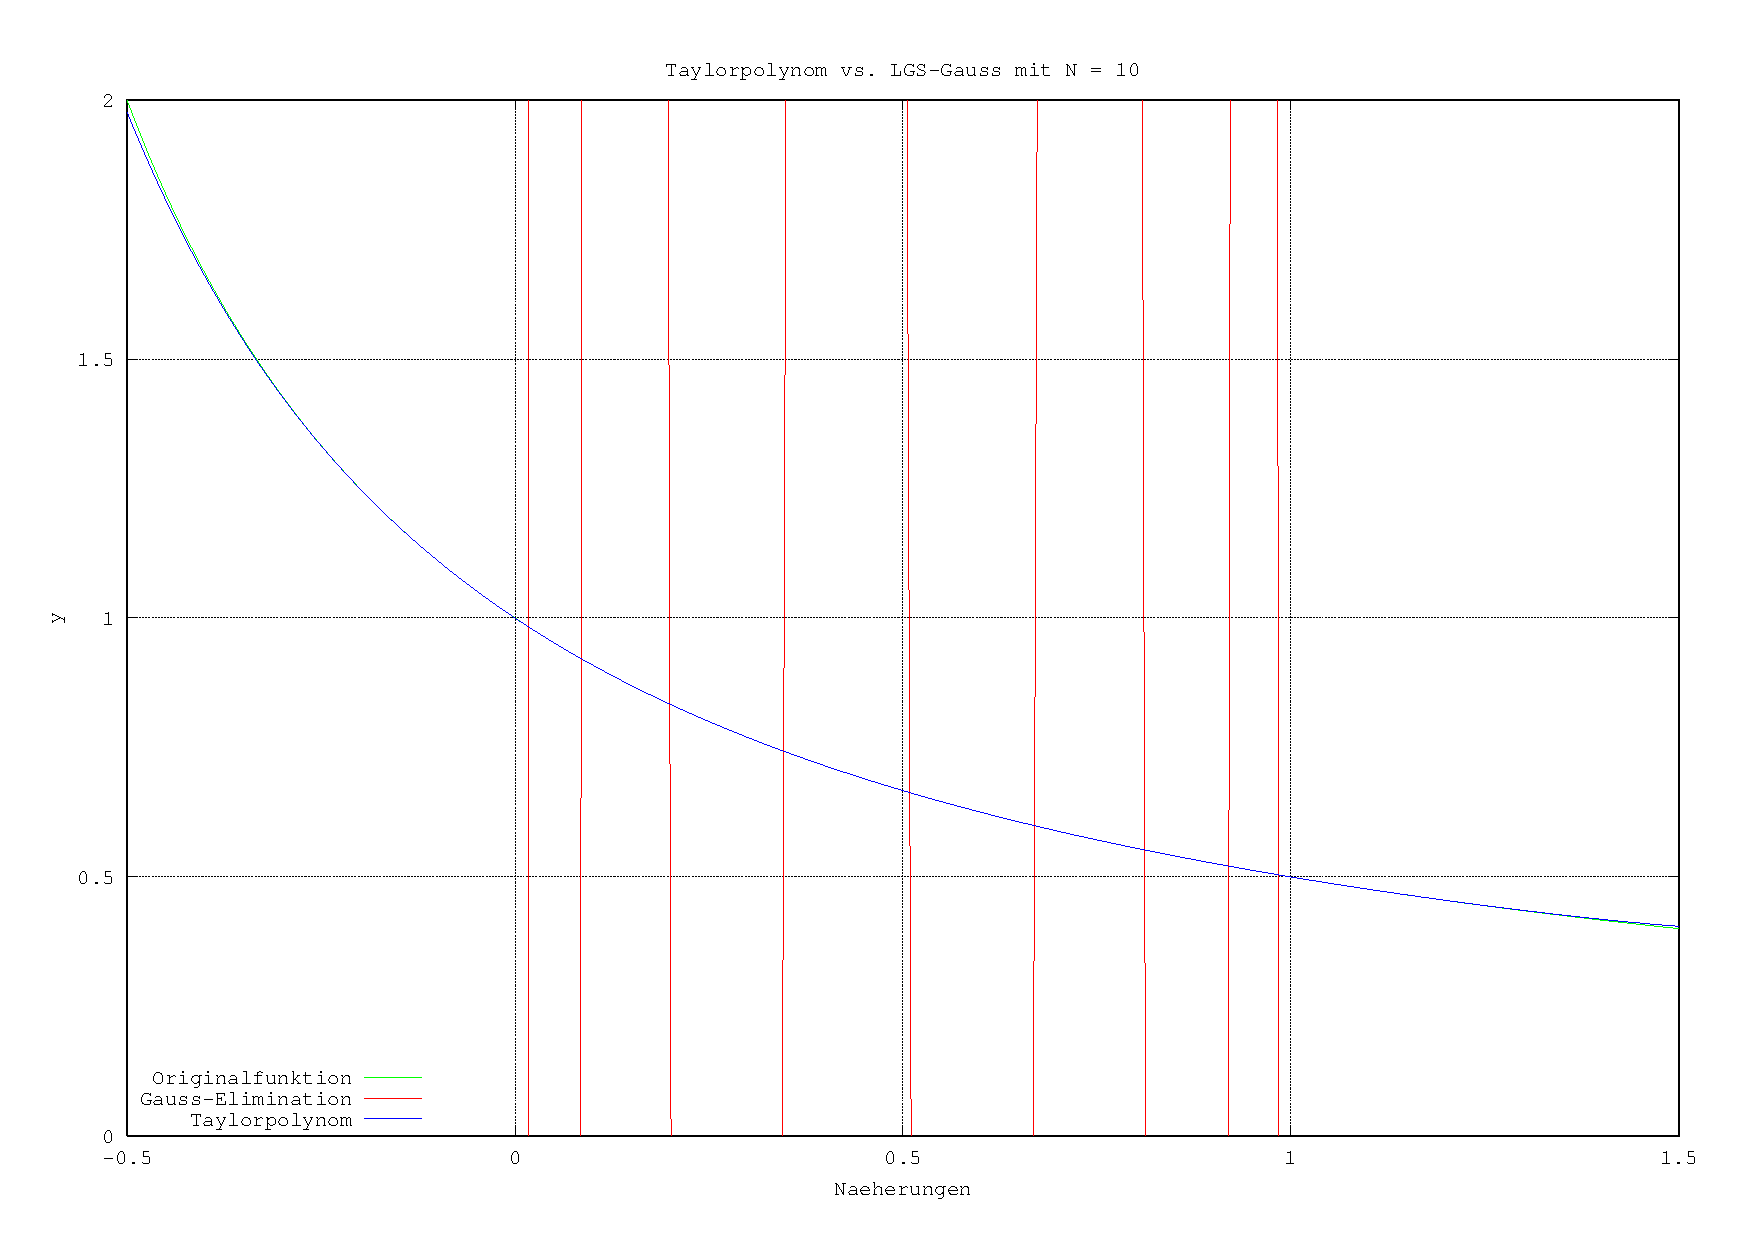
\includegraphics[width=\textwidth]{img/aufgabe5.pdf}
    \end{center}
    \vspace{-1em}
    \caption{Plot des Taylorpolynoms vs. Gauss-Elimination}
    \label{fig:TaylorVsGauss}
\end{figure}

\section{Ausblick}
Um das schlecht konditionierte Gleichungssystem dennoch lösen zu können, bietet sich das
Regularisierungsverfahren nach Tikhonov\footnote{Andrei Nikolajewitsch Tichonow (russisch Андрей
Николаевич Тихонов, wiss. Transliteration Andrej Nikolaevič Tichonov; englische Transliteration
Andrei Tikhonov; * 17. Oktoberjul./ 30. Oktober 1906greg. in Gschatsk; † 7. November 1993 in Moskau)
war ein russischer Mathematiker. Oft wird auch die Schreibung Tychonoff verwendet} an. An dieser
stelle soll jedoch dieses nicht weiter erläutert, sondern nur dessen Implementierung in Octave
aufgezeigt werden. Für das Listing siehe \ref{code:tikhonov} das hiermit resultierende Polynom ist
in Abbildung \ref{fig:Tikonov} zu sehen.

\begin{figure}[H]
    \vspace{-1em}
    \begin{center}
        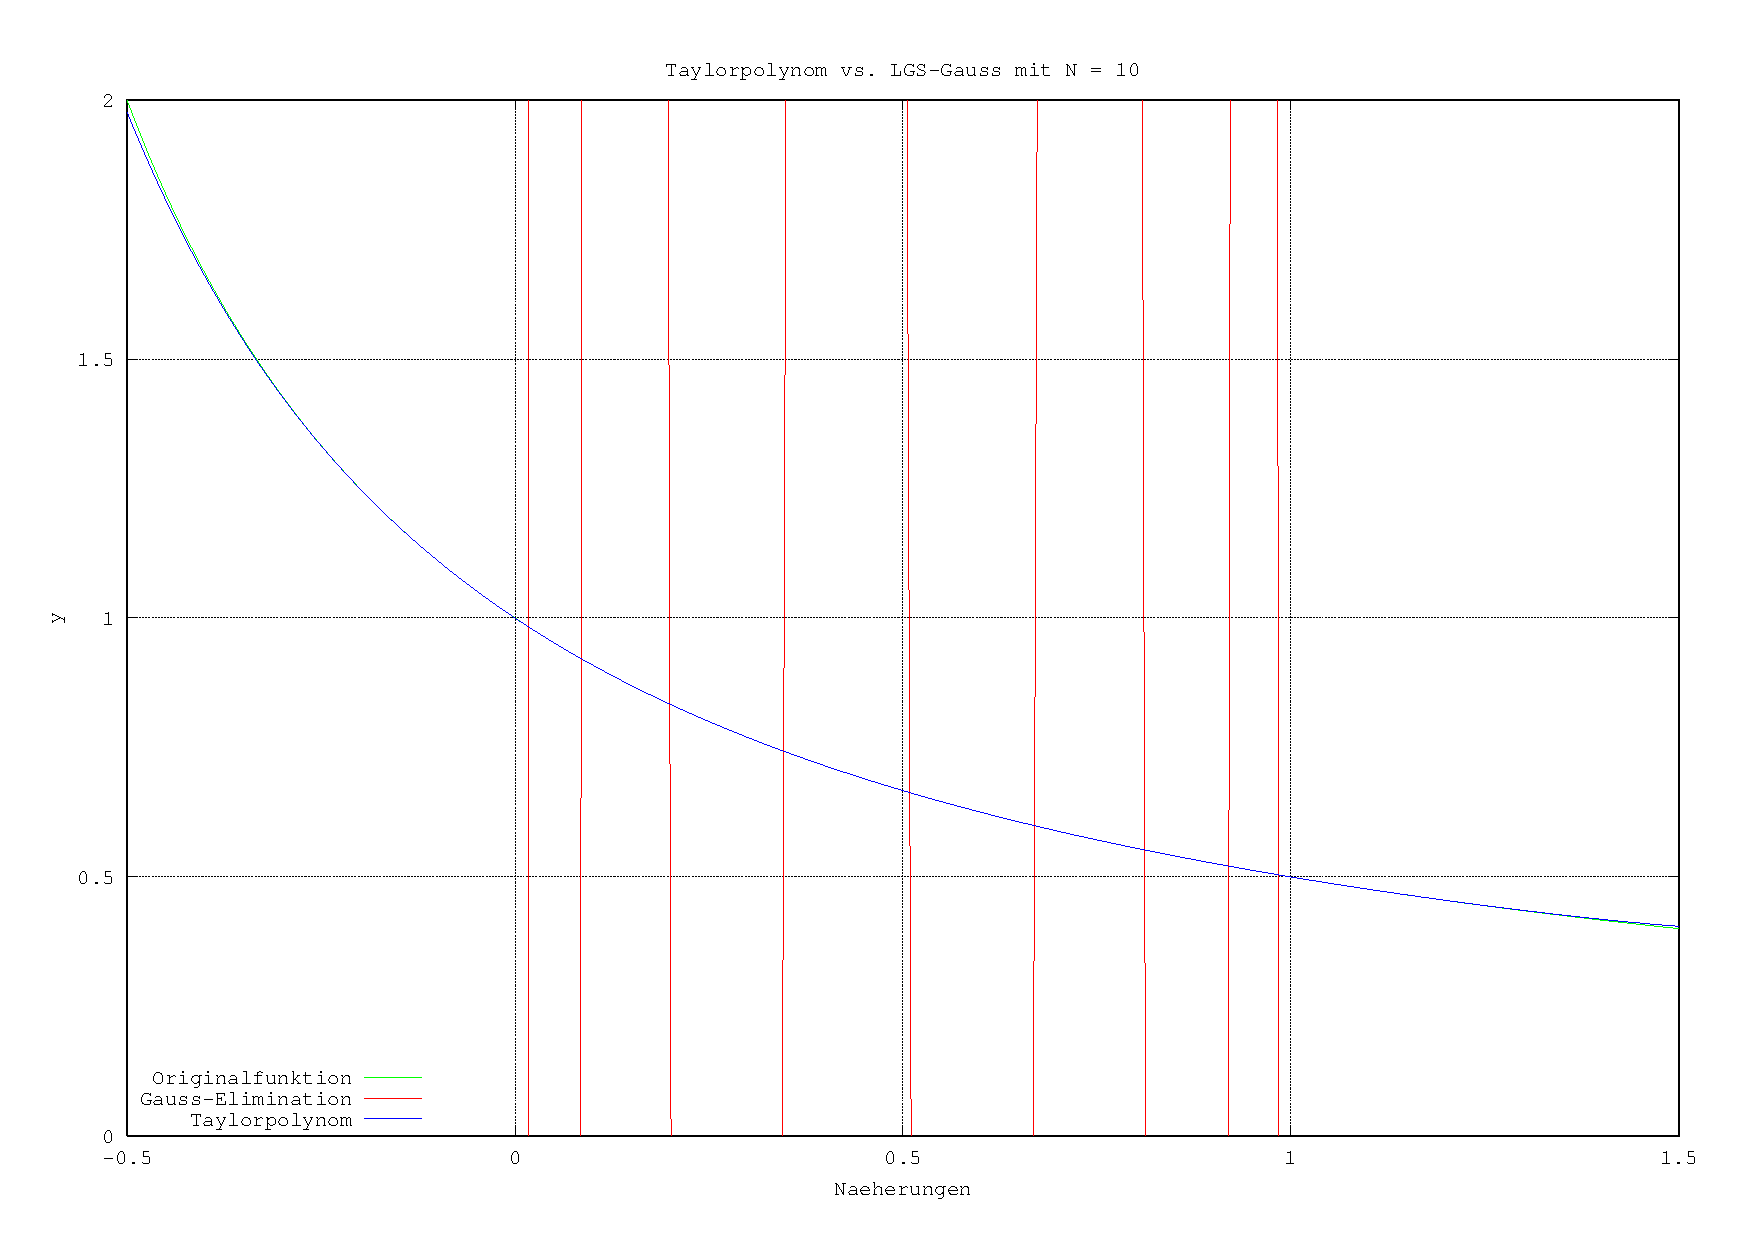
\includegraphics[width=\textwidth]{img/aufgabe5.pdf}
    \end{center}
    \vspace{-1em}
    \caption{Plot der Tikhonov Regularisierung}
    \label{fig:Tikonov}
\end{figure}